% TEMPLATE for Usenix papers, specifically to meet requirements of
%  USENIX '05
% originally a template for producing IEEE-format articles using LaTeX.
%   written by Matthew Ward, CS Department, Worcester Polytechnic Institute.
% adapted by David Beazley for his excellent SWIG paper in Proceedings,
%   Tcl 96
% turned into a smartass generic template by De Clarke, with thanks to
%   both the above pioneers
% use at your own risk.  Complaints to /dev/null.
% make it two column with no page numbering, default is 10 point

% Munged by Fred Douglis <douglis@research.att.com> 10/97 to separate
% the .sty file from the LaTeX source template, so that people can
% more easily include the .sty file into an existing document.  Also
% changed to more closely follow the style guidelines as represented
% by the Word sample file. 

% Note that since 2010, USENIX does not require endnotes. If you want
% foot of page notes, don't include the endnotes package in the 
% usepackage command, below.

\documentclass[letterpaper,twocolumn,10pt]{article}
\usepackage{usenix,epsfig,endnotes}
\begin{document}

%don't want date printed
\date{}

%make title bold and 14 pt font (Latex default is non-bold, 16 pt)
\title{\Large \bf Security and Efficiency of an Open Wireless Campus Network}

\author{
{\rm Christian D.\ Tuen}\\
UCSB Graduate Student\\
christiandt@umail.ucsb.edu
\and
{\rm Kine Johnsrud}\\
UCSB Graduate Student\\
kinej@umail.ucsb.edu
\and
{\rm Andreas L\o{}vland}\\
UCSB Graduate Student\\
asl@umail.ucsb.edu
}
\maketitle

% Use the following at camera-ready time to suppress page numbers.
% Comment it out when you first submit the paper for review.
\thispagestyle{empty}

\subsection*{Abstract}
Having a WLAN (Wireless Local Area Network) is now so commonplace in academic campuses, that it is more or less taken for granted by its users. Hence, it is increasingly important to understand usage and usage-changes in a technological world that is rapidly changing.

In this paper, we want to take a look at the general usage, efficiency and security of a campus network as a whole, by using passive network monitoring software. Over a span of 5 weekdays we detected 956 unique devices at the UCSB Davidson Library, by monitoring for two hours daily.

We found that there is a large increase in use of mobile OSes since earlier studies~\cite{Campus2004}, and that OSX has superseded Windows. We observed that some of the most used applications are media-heavy, and that the campus network might not handle the pressure. We also observed that half the traffic being transferred over the unsecured network is secured by means of SSL. We discovered trends in what websites were visited the most, and what application are most widely used. Lastly, we found that there was a substantial amount of control packages, in addition to retransmission-packages and faulty packages, making for a relative low general goodput.

\section{Introduction}

In this day and age WiFi connectivity is taken for granted, and the number of mobile devices per person has rapidly increased in the later years. Public companies and institutions are not always the first to adapt to rapidly increasing usage of such wireless networks. In this paper we conduct a study of todays usage of a campus network, and talk about how well the network performs. University of California Santa Barbara (UCSB) has recently launched its secure wireless network, but many students are still using the unsecured one.

Firstly, we show what operating systems are used now, and how many of them are on the emerging mobile platform. This is set in comparison to a paper analyzing a campus-network in 2004~\cite{Campus2004}. We also analyze whether there are any obvious usage patterns, i.e. if we can get a strong top 10 websites visited and applications used. Since this is an unsecured network, it is also interesting to see whether the connections are generally secured, and whether they are secured well.

This is a network that has a large user base, and the library is often densely packed with people and devices. This led us to believe that this network might be congested, especially at given access points. We show how much of the channel is used to send control packets, as well as analyzing whether packets sent can be considered as goodput (not being retransmissions or faulty packets). Our findings show that the network might be a bit congested, and assume that this is due to a large user base, and a lot of obstacles and movement.

We next describe the environment of our study, the UCSB Davidson Library, and how we conducted our data collection period. In section 3 we present our results of the operating systems comparison, then and now. In section 4 we talk about the security aspect of an open wireless network, and show some performance metrics comparing the secured and unsecured connections. Section 5 shows the usage patterns of the students using this network, by means of websites requested and applications used. In section 6 we discuss our findings regarding the amount of control packages sent in the network, as well as how much of the data sent is actual goodput. The paper gets wrapped up with a conclusion in section 7.

\section{Test environment and trace collection}

The UCSB Davidson Library is of medium size, and is generally full of people. Observation shows that it is reasonable to assume that all students own a laptop, and many students own one or more other mobile devices in addition (smartphone, tablet, etc.). 

The passive monitoring were performed using personal computers, sitting in the same spot in the library each day of the experiment. It was done Monday through Friday in week 43, between 1pm and 3pm. The data was not stripped down to only containing headers, and the complete raw dataset ended up being 26 GB. We did the capturing with two different devices (A Mac and a Linux machine). In hindsight we would have done differently because we have had some compatibility issues, but in general we still think our results are correct and presentable.

We expected to see a wide variety of devices connected, ranging from Mac and Windows PCs, to a wide variety of smartphones and tablets.

\begin{figure}[!htb] 
\begin{center} 
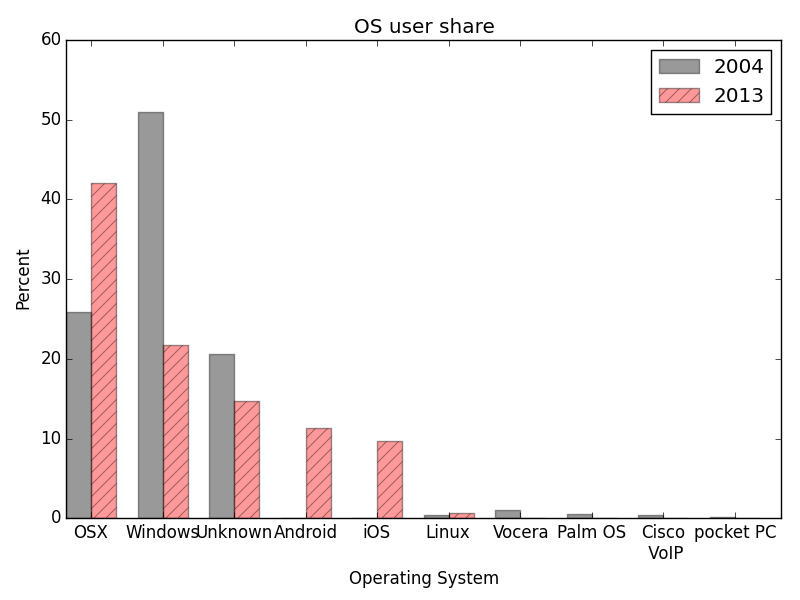
\includegraphics[width=3in]{os.png} 
\caption{Distribution of Operating Systems} 
\label{fig:os} 
\end{center} 
\end{figure}

\section{Operating Systems}

An inspiration for writing this paper is a research paper from 2004 doing an extensive analysis of a campus-wide network~\cite{Campus2004}. They have made a table showing all the devices(operating systems) seen on the wireless network. They used a passive OS fingerprinting tool named p0f~\cite{p0f}, and we started of with that as well. However, the tool is a bit outdated, and we chose to find the operating systems ourselves by looking at the User Agent fields in the request-packets.
 
This was before the smartphone-era, and in figure~\ref{fig:os} we can see the changes in operating systems and devices between now and 2004. In addition to Apples OSX superseding Microsofts Windows, we now have mobile platforms (android and iOS) taking up 20 \% of the total. Even though the emerging mobile market is a well known fact by now, it is highly interesting to see its effect on wireless networks and its performance. We will explore this further in subsection 6.2.

\section{Security and performance}

In this section we present the security aspect of an open wireless network, and take a look at the performance differences between secured and unsecured connections.

\begin{table}
\footnotesize
    \begin{tabular}{|p{6.3cm}|l|}
    \hline
     			{\bf Encryption Type}                      &  			{\bf Percent} \\ \hline
     			TLS\_RSA\_WITH\_AES\_128\_CBC\_SHA    &  			29.97\% \\ \hline
     			TLS\_ECDHE\_RSA\_WITH\_RC4\_128\_SHA  &  			17.63\% \\ \hline
     			TLS\_RSA\_WITH\_AES\_256\_CBC\_SHA    &  			13.83\% \\ \hline
     			TLS\_RSA\_WITH\_RC4\_128\_SHA         &  			11.79\% \\ \hline
     			TLS\_RSA\_WITH\_RC4\_128\_MD5         &  			9.40\%  \\ \hline
     			TLS\_ECDHE\_ECDSA\_WITH\_RC4\_128\_SHA &  			6.32\%  \\ \hline
     			TLS\_DHE\_RSA\_WITH\_AES\_256\_CBC\_SHA &  			3.80\%  \\ \hline
     			TLS\_ECDHE\_RSA\_WITH\_AES\_128\_CBC\_SHA &  			3.45\%  \\ \hline
     			TLS\_ECDHE\_RSA\_WITH\_AES\_256\_CBC\_SHA &  			0.92\%  \\ \hline
     			TLS\_DHE\_RSA\_WITH\_CAMELLIA\_256\_CBC\_SHA &  			0.76\%  \\ \hline
    \end{tabular}
    \caption{List of cryptographic suites and their usage}
    \label{tab:encryptions}
\end{table}

\subsection{Security}

From our dataset, we found that 62 \% of the connections were unsecured HTTP-sessions, and the other 38 \% connections were secured by SSL/HTTPS. The increasing use of HTTPS-connections can be assumed to be an effect of popular social websites like Facebook and Twitter securing their sites by default.

A secured connection that is secured badly is often worse than an unsecured connection, since sensitive information often is the reason for securing the connection in the first place. We therefore found it reasonable to investigate whether the cryptographic suites used were properly secure. The cryptographic suites used is shown in table~\ref{tab:encryptions}, and they are all considered secure enough by the Standards Organizations~\cite{NIST}. This is natural considering the new enthusiasm for privacy and security, and the fact that the biggest and most used websites needs to be properly secured to keep their reputation.

\begin{figure*}[!htb] 
\begin{center} 
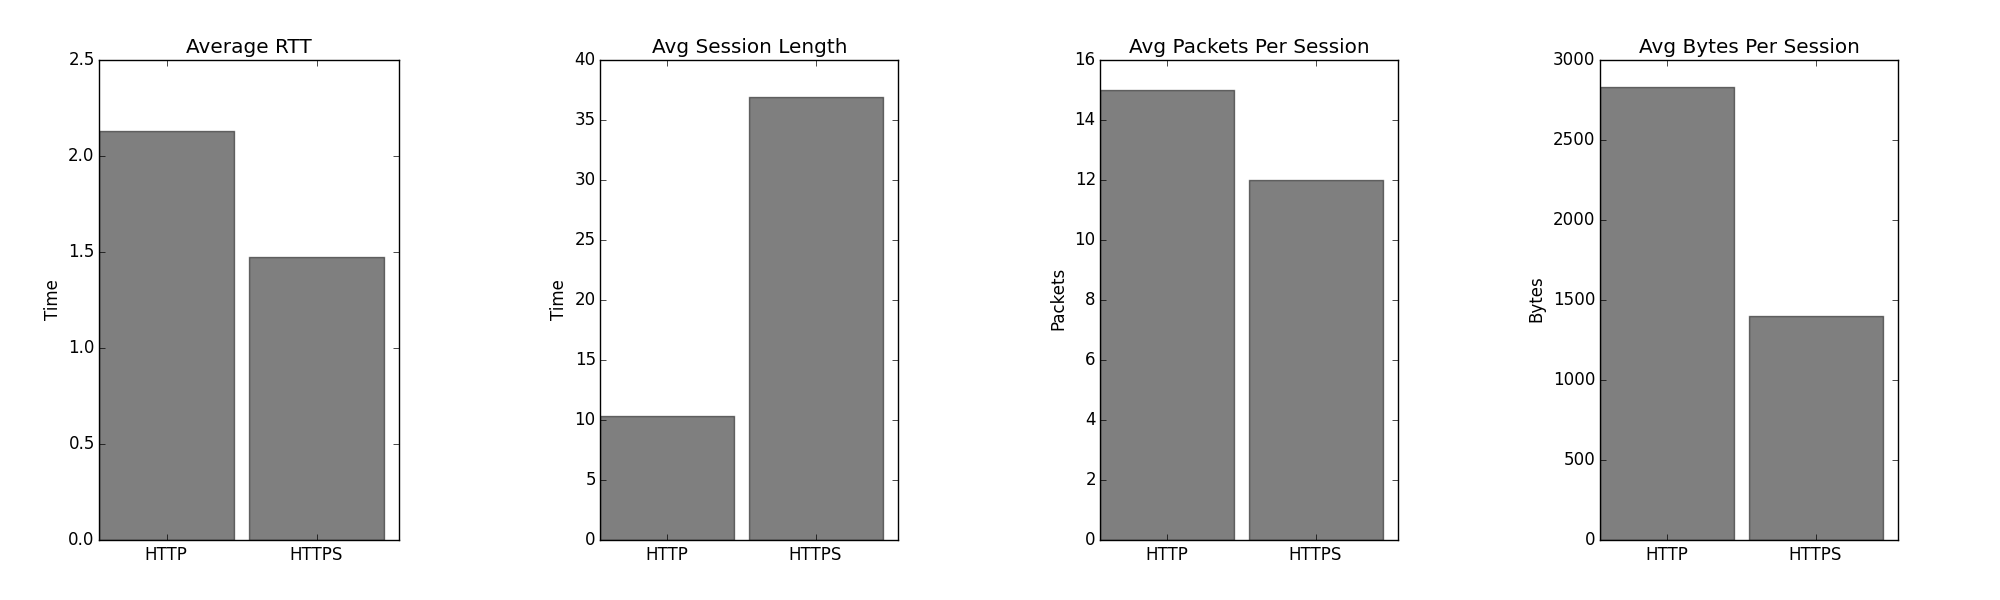
\includegraphics[width=7in]{combined.png} 
\caption{HTTP and HTTPS differences compared to RTT, average session length, average number of packets per session and average number of bytes per session} 
\label{fig:combined}
\end{center} 
\end{figure*}

\subsection{Performance}

When using SSL, there is reason to believe that there will be a difference in performance. Other studies~\cite{SSL} show that there is a performance-loss when using SSL, because time and processing power is used to encrypt and decrypt. In figure~\ref{fig:combined}, we see that average Round-Trip-Time is in fact larger for HTTP than HTTPS. This can be a cause of various reasons, but shows that there is not a noticeable difference between the two. Average session length is more than three times longer with HTTPS. This is natural, as the servers would like to keep the encrypted connection for a longer period of time, and not having to renegotiate cryptographic suites.

From the two graphs on the right in figure~\ref{fig:combined}, we can see that HTTP has more than double the average amount of bytes per session than HTTPS, even though the average number of packets per session is close to equal between the two. This might be explained by the fact that a lot of video streams (youtube, gauchocast) are sent unsecured, and a lot of secured links are simple websites like Facebook and Twitter, as well as mail services.

\section{Usage: Web sites and application}

To better understand the usage of a wireless network, it is essential to take a look at what the users are actually doing on the wifi, as well as what the devices are doing without a user noticing it. In this section we will take a look at popular websites, and what applications are using the network. By applications, we count desktop-applications as well as mobile.

\begin{figure}[!htb] 
\begin{center} 
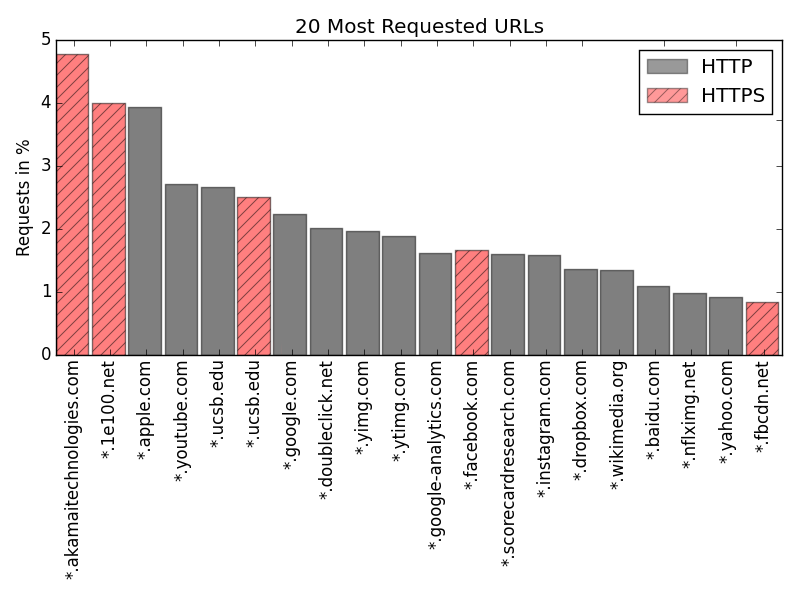
\includegraphics[width=3in]{websites.png} 
\caption{The 20 most requested URLs, color coded by their use of HTTPS or HTTP} 
\label{fig:websites} 
\end{center} 
\end{figure}

\subsection{Web sites}

In relation to usage-patterns, we initially hoped to get a clear top 10 list of the most popular websites out there in number of requests. We count both the number of HTTP requests, and HTTPS requests by doing a reverse DNS lookup on the "server hello"-source address. As the results have a long tail and a slow drop off, we included the top 20 URLs in our analyzation shown in figure~\ref{fig:websites}. These 20 URLs account for 41.69 \% of all HTTP/HTTPS requests, and should provide a good picture of usage. Most of the URLs are CDNs, which correlates with how CDNs are used in general. For instance, in a sample test, ytimg.com was requested more than 20 times when loading the YouTube frontpage. 

If we look at the URLs in terms of web pages, we see that most have two or more occurrences in the list. The reason for this is that bigger companies, handling many requests per second, are only encrypting data that needs to be encrypted while sending data that do not need to be encrypted on unencrypted connections as encryption adds processing load on the servers. All of the sites that are not hidden behind "Akamai" are either social websites, school related, advertisements or file/video/image related.

\begin{figure}[!htb] 
\begin{center} 
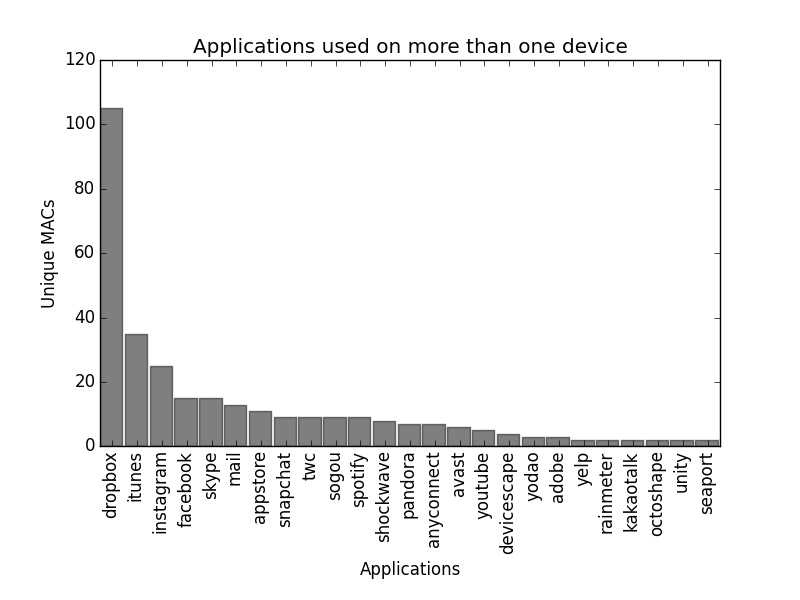
\includegraphics[width=3.3in]{applications.png} 
\caption{Distribution of unique MAC addresses per application} 
\label{fig:applications} 
\end{center}
\end{figure}

\subsection{Applications}

To retrieve information about applications, we used the HTTP-requests User Agent field. Even though a lot of applications use an encrypted connection to the backend API, most applications also connect to third party unencrypted analytics services. This way, we will still see an HTTP request from these applications, and be able to gather User Agent data from the devices.

In figure~\ref{fig:applications}, we show the number of unique MAC-addresses sending HTTP-request with application-information. For readability, we choose to show the applications used by more than one single device. This graph shows that the most used applications are all media-heavy applications potentially consuming a lot of the bandwidth. The top application is Dropbox, that automatically downloads new and modified files in the background. Daemon processes running in the background which the user is potentially unaware of, consumes a lot of the bandwidth that could have been used more effectively for other purposes.

\section{Control Packets}

In trying to understand whether this network is congested or not, it is natural to find out about the ratio between control packets and data packets in general, as well as goodput versus throughput. Throughput is all data sent, including retransmissions and overhead, while goodput is actual useful data received at application level. In this section we will first look at goodput vs. throughput, followed by focusing on sending of RTS and CTS packets.

\subsection{Goodput vs. Throughput}

When looking into what of the data is considered goodput, we also have to take packet loss and retransmissions into account, as well as flawed packets. This amounts to 68 \% of the packets not being goodput, and one third of all the bytes sent (figure~\ref{fig:goodput_combined}). In other words, only two thirds of all data sent are useful information. This can both indicate a congested network, as well as a network with a lot of conflicting noise. With many people gathered in a small space trying to make many requests at the same time, this is a reasonable assumption to make. The library is highly used by the universitys students, and due to construction work the library has less space available than usual.

To get a perspective, we found that around 56 \% of the data sent was control packets, but due to the relative small size of control packets, it only added up to about 10 \% of the total data traffic (figure~\ref{fig:control_combined}). This indicates that a large amount of the flawed data sent on this network is retransmitted packages, and flawed packages (with checksum error).

\begin{figure}[!htb] 
\begin{center} 
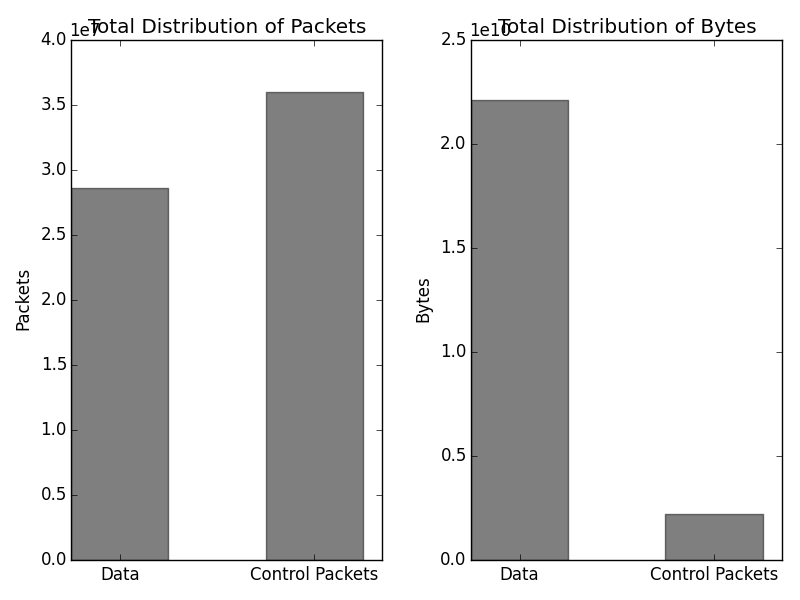
\includegraphics[width=3in]{control_combined.png} 
\caption{Left: The number of control packets compared to data packets. Right: The number of bytes generated by data and control packets} 
\label{fig:control_combined} 
\end{center} 
\end{figure}

\begin{figure}[!htb] 
\begin{center} 
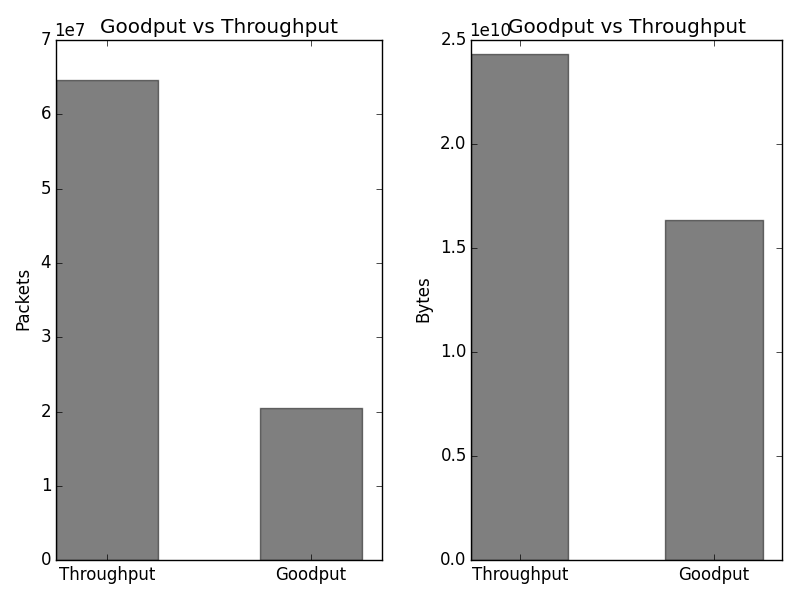
\includegraphics[width=3in]{goodput_combined.png} 
\caption{Left: Goodput versus Throughput in term of packets. Right: Goodput versus Throughput in term of bytes} 
\label{fig:goodput_combined} 
\end{center} 
\end{figure}

\subsection{RTS \& CTS}

Request-to-Send and Clear-to-Send is an 802.11 mechanism used to reduce frame collisions due to hidden terminal problem. The use of this mechanism is a good fairness-idea, but is often disabled by default in most wireless cards. However, we found that the average amount of RTS and CTS packets sent, were as high as 5 \% of the total number of packets. We decided to investigate this further.

We did a lookup of the MAC addresses sending the RTS and CTS packets, and based on vendor (figure~\ref{fig:rtscts_vendor}), it was obvious that this was mainly the Cisco Access Points using this function, but also mobile devices. After Cisco, the top three MAC adresses were from HonHai, LiteOn and Apple. These are all companies making mobile devices (Apple), or making chips used in a variety of smartphones (HonHai, LiteOn). A little research showed that RTS and CTS or CTS-to-Self is something that many smartphones use when WiFi is enabled. Other studies~\cite{Smartphones} has used this fact to track wifi-enabled smartphones.

\begin{figure}[!htb] 
\begin{center} 
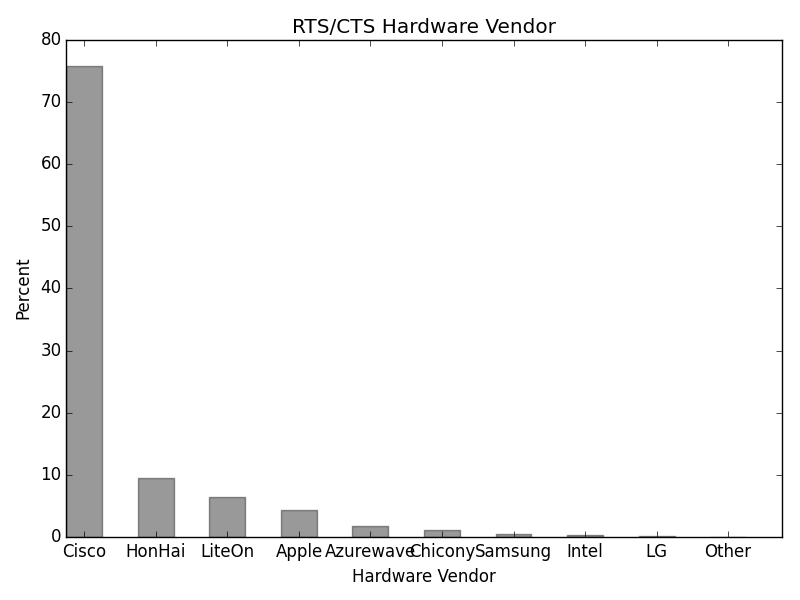
\includegraphics[width=3in]{rtscts_vendor.png} 
\caption{Percentage of unique MAC addresses that has sent RTS or CTS, grouped by vendor} 
\label{fig:rtscts_vendor} 
\end{center} 
\end{figure}

\section{Conclusion}
We conducted a study of a campus wireless network, in an effort to understand mechanisms and patterns of activity in the network. It is important to remember the context - our results stem from a population of university students, and may not be relatable to corporate firms or other public space venues.

During the hours of capturing, the traffic was constantly high and a large set of clients were connected at all times during these two-hour periods.

We were able to subtract information about what operating systems people used, and then also finding out how many of the connected devices were smartphones and tablets. This was put into perspective and compared to a study from 2004.

We were able to figure out how much data is sent over SSL, and what cryptographic schemes they used. We also concluded that they were all considered safe by the Standards Organizations. To see usage-patterns, we made a list of the top 20 most visited URLs on the Internet, and found out that URL-requests are usually for social websites, university-related, advertisement or video-streaming. When it comes to application-usage, we found that most of the applications with highest user base, are also applications with media-content and generally large files being synced or streamed over the network.

Lastly, we did a study of control packets, to better understand whether the network was performing well or not. 56 \% of all packets sent were control packages, but due to their small size it was only about 9 \% of the total number of bytes sent. More alarmingly, we found that only two thirds of the data sent is what we consider goodput. With so many users trying to make requests at the same time at such a small place, this is to be expected. The library is heavily used by the universitys students, and due to construction work the library has less space available than usual.

\section{Related Work}

Our study is a small scale and passive measurement of a single point in a campus network. There are many similar and larger scale studies looking at these kind of characteristics. Henderson et al~\cite{Campus2004} did an extensive network trace including more than 550 access points and 7000 users over seventeen weeks. This kind of study would be impossible for us to make, but we were still able to compare some of our data. Similar to that campus-study, is a study by Kotz et al~\cite{Campus2002} using a campus-wide network of 476 access points spread over 161 buildings.

In studying whether the network performs different whether SSL is used or not, Vicen\c{c} et al~\cite{SSL} has done an extensive study over the computational and resource demand of encryption and decryption of data. Senad et al~\cite{Campus2011} has done an extensive vulnerability study of the security architecture of a campus network. Even though we have only been able to study the security between end-user and access point, the security aspect of a university network is highly important and interesting.


{\footnotesize \bibliographystyle{acm}
\bibliography{sample}}


%\theendnotes

\end{document}







